% Options for packages loaded elsewhere
\PassOptionsToPackage{unicode}{hyperref}
\PassOptionsToPackage{hyphens}{url}
\PassOptionsToPackage{dvipsnames,svgnames,x11names}{xcolor}
%
\documentclass[
  letterpaper,
  DIV=11,
  numbers=noendperiod]{scrartcl}

\usepackage{amsmath,amssymb}
\usepackage{iftex}
\ifPDFTeX
  \usepackage[T1]{fontenc}
  \usepackage[utf8]{inputenc}
  \usepackage{textcomp} % provide euro and other symbols
\else % if luatex or xetex
  \usepackage{unicode-math}
  \defaultfontfeatures{Scale=MatchLowercase}
  \defaultfontfeatures[\rmfamily]{Ligatures=TeX,Scale=1}
\fi
\usepackage{lmodern}
\ifPDFTeX\else  
    % xetex/luatex font selection
\fi
% Use upquote if available, for straight quotes in verbatim environments
\IfFileExists{upquote.sty}{\usepackage{upquote}}{}
\IfFileExists{microtype.sty}{% use microtype if available
  \usepackage[]{microtype}
  \UseMicrotypeSet[protrusion]{basicmath} % disable protrusion for tt fonts
}{}
\makeatletter
\@ifundefined{KOMAClassName}{% if non-KOMA class
  \IfFileExists{parskip.sty}{%
    \usepackage{parskip}
  }{% else
    \setlength{\parindent}{0pt}
    \setlength{\parskip}{6pt plus 2pt minus 1pt}}
}{% if KOMA class
  \KOMAoptions{parskip=half}}
\makeatother
\usepackage{xcolor}
\setlength{\emergencystretch}{3em} % prevent overfull lines
\setcounter{secnumdepth}{-\maxdimen} % remove section numbering
% Make \paragraph and \subparagraph free-standing
\makeatletter
\ifx\paragraph\undefined\else
  \let\oldparagraph\paragraph
  \renewcommand{\paragraph}{
    \@ifstar
      \xxxParagraphStar
      \xxxParagraphNoStar
  }
  \newcommand{\xxxParagraphStar}[1]{\oldparagraph*{#1}\mbox{}}
  \newcommand{\xxxParagraphNoStar}[1]{\oldparagraph{#1}\mbox{}}
\fi
\ifx\subparagraph\undefined\else
  \let\oldsubparagraph\subparagraph
  \renewcommand{\subparagraph}{
    \@ifstar
      \xxxSubParagraphStar
      \xxxSubParagraphNoStar
  }
  \newcommand{\xxxSubParagraphStar}[1]{\oldsubparagraph*{#1}\mbox{}}
  \newcommand{\xxxSubParagraphNoStar}[1]{\oldsubparagraph{#1}\mbox{}}
\fi
\makeatother

\usepackage{color}
\usepackage{fancyvrb}
\newcommand{\VerbBar}{|}
\newcommand{\VERB}{\Verb[commandchars=\\\{\}]}
\DefineVerbatimEnvironment{Highlighting}{Verbatim}{commandchars=\\\{\}}
% Add ',fontsize=\small' for more characters per line
\usepackage{framed}
\definecolor{shadecolor}{RGB}{241,243,245}
\newenvironment{Shaded}{\begin{snugshade}}{\end{snugshade}}
\newcommand{\AlertTok}[1]{\textcolor[rgb]{0.68,0.00,0.00}{#1}}
\newcommand{\AnnotationTok}[1]{\textcolor[rgb]{0.37,0.37,0.37}{#1}}
\newcommand{\AttributeTok}[1]{\textcolor[rgb]{0.40,0.45,0.13}{#1}}
\newcommand{\BaseNTok}[1]{\textcolor[rgb]{0.68,0.00,0.00}{#1}}
\newcommand{\BuiltInTok}[1]{\textcolor[rgb]{0.00,0.23,0.31}{#1}}
\newcommand{\CharTok}[1]{\textcolor[rgb]{0.13,0.47,0.30}{#1}}
\newcommand{\CommentTok}[1]{\textcolor[rgb]{0.37,0.37,0.37}{#1}}
\newcommand{\CommentVarTok}[1]{\textcolor[rgb]{0.37,0.37,0.37}{\textit{#1}}}
\newcommand{\ConstantTok}[1]{\textcolor[rgb]{0.56,0.35,0.01}{#1}}
\newcommand{\ControlFlowTok}[1]{\textcolor[rgb]{0.00,0.23,0.31}{\textbf{#1}}}
\newcommand{\DataTypeTok}[1]{\textcolor[rgb]{0.68,0.00,0.00}{#1}}
\newcommand{\DecValTok}[1]{\textcolor[rgb]{0.68,0.00,0.00}{#1}}
\newcommand{\DocumentationTok}[1]{\textcolor[rgb]{0.37,0.37,0.37}{\textit{#1}}}
\newcommand{\ErrorTok}[1]{\textcolor[rgb]{0.68,0.00,0.00}{#1}}
\newcommand{\ExtensionTok}[1]{\textcolor[rgb]{0.00,0.23,0.31}{#1}}
\newcommand{\FloatTok}[1]{\textcolor[rgb]{0.68,0.00,0.00}{#1}}
\newcommand{\FunctionTok}[1]{\textcolor[rgb]{0.28,0.35,0.67}{#1}}
\newcommand{\ImportTok}[1]{\textcolor[rgb]{0.00,0.46,0.62}{#1}}
\newcommand{\InformationTok}[1]{\textcolor[rgb]{0.37,0.37,0.37}{#1}}
\newcommand{\KeywordTok}[1]{\textcolor[rgb]{0.00,0.23,0.31}{\textbf{#1}}}
\newcommand{\NormalTok}[1]{\textcolor[rgb]{0.00,0.23,0.31}{#1}}
\newcommand{\OperatorTok}[1]{\textcolor[rgb]{0.37,0.37,0.37}{#1}}
\newcommand{\OtherTok}[1]{\textcolor[rgb]{0.00,0.23,0.31}{#1}}
\newcommand{\PreprocessorTok}[1]{\textcolor[rgb]{0.68,0.00,0.00}{#1}}
\newcommand{\RegionMarkerTok}[1]{\textcolor[rgb]{0.00,0.23,0.31}{#1}}
\newcommand{\SpecialCharTok}[1]{\textcolor[rgb]{0.37,0.37,0.37}{#1}}
\newcommand{\SpecialStringTok}[1]{\textcolor[rgb]{0.13,0.47,0.30}{#1}}
\newcommand{\StringTok}[1]{\textcolor[rgb]{0.13,0.47,0.30}{#1}}
\newcommand{\VariableTok}[1]{\textcolor[rgb]{0.07,0.07,0.07}{#1}}
\newcommand{\VerbatimStringTok}[1]{\textcolor[rgb]{0.13,0.47,0.30}{#1}}
\newcommand{\WarningTok}[1]{\textcolor[rgb]{0.37,0.37,0.37}{\textit{#1}}}

\providecommand{\tightlist}{%
  \setlength{\itemsep}{0pt}\setlength{\parskip}{0pt}}\usepackage{longtable,booktabs,array}
\usepackage{calc} % for calculating minipage widths
% Correct order of tables after \paragraph or \subparagraph
\usepackage{etoolbox}
\makeatletter
\patchcmd\longtable{\par}{\if@noskipsec\mbox{}\fi\par}{}{}
\makeatother
% Allow footnotes in longtable head/foot
\IfFileExists{footnotehyper.sty}{\usepackage{footnotehyper}}{\usepackage{footnote}}
\makesavenoteenv{longtable}
\usepackage{graphicx}
\makeatletter
\newsavebox\pandoc@box
\newcommand*\pandocbounded[1]{% scales image to fit in text height/width
  \sbox\pandoc@box{#1}%
  \Gscale@div\@tempa{\textheight}{\dimexpr\ht\pandoc@box+\dp\pandoc@box\relax}%
  \Gscale@div\@tempb{\linewidth}{\wd\pandoc@box}%
  \ifdim\@tempb\p@<\@tempa\p@\let\@tempa\@tempb\fi% select the smaller of both
  \ifdim\@tempa\p@<\p@\scalebox{\@tempa}{\usebox\pandoc@box}%
  \else\usebox{\pandoc@box}%
  \fi%
}
% Set default figure placement to htbp
\def\fps@figure{htbp}
\makeatother

\KOMAoption{captions}{tableheading}
\makeatletter
\@ifpackageloaded{caption}{}{\usepackage{caption}}
\AtBeginDocument{%
\ifdefined\contentsname
  \renewcommand*\contentsname{Table of contents}
\else
  \newcommand\contentsname{Table of contents}
\fi
\ifdefined\listfigurename
  \renewcommand*\listfigurename{List of Figures}
\else
  \newcommand\listfigurename{List of Figures}
\fi
\ifdefined\listtablename
  \renewcommand*\listtablename{List of Tables}
\else
  \newcommand\listtablename{List of Tables}
\fi
\ifdefined\figurename
  \renewcommand*\figurename{Figure}
\else
  \newcommand\figurename{Figure}
\fi
\ifdefined\tablename
  \renewcommand*\tablename{Table}
\else
  \newcommand\tablename{Table}
\fi
}
\@ifpackageloaded{float}{}{\usepackage{float}}
\floatstyle{ruled}
\@ifundefined{c@chapter}{\newfloat{codelisting}{h}{lop}}{\newfloat{codelisting}{h}{lop}[chapter]}
\floatname{codelisting}{Listing}
\newcommand*\listoflistings{\listof{codelisting}{List of Listings}}
\makeatother
\makeatletter
\makeatother
\makeatletter
\@ifpackageloaded{caption}{}{\usepackage{caption}}
\@ifpackageloaded{subcaption}{}{\usepackage{subcaption}}
\makeatother

\usepackage{bookmark}

\IfFileExists{xurl.sty}{\usepackage{xurl}}{} % add URL line breaks if available
\urlstyle{same} % disable monospaced font for URLs
\hypersetup{
  pdftitle={The Geometry of Categorical and Hierarchical Concepts in Large Language Models},
  pdfauthor={Kiho Park, Yo Joong Choe, Yibo Jiang, and Victor Veitch},
  colorlinks=true,
  linkcolor={blue},
  filecolor={Maroon},
  citecolor={Blue},
  urlcolor={Blue},
  pdfcreator={LaTeX via pandoc}}


\title{The Geometry of Categorical and Hierarchical Concepts in Large
Language Models}
\author{Kiho Park, Yo Joong Choe, Yibo Jiang, and Victor Veitch}
\date{}

\begin{document}
\maketitle


\section{Background}\label{background}

\subsection{LLM Background}\label{llm-background}

\pandocbounded{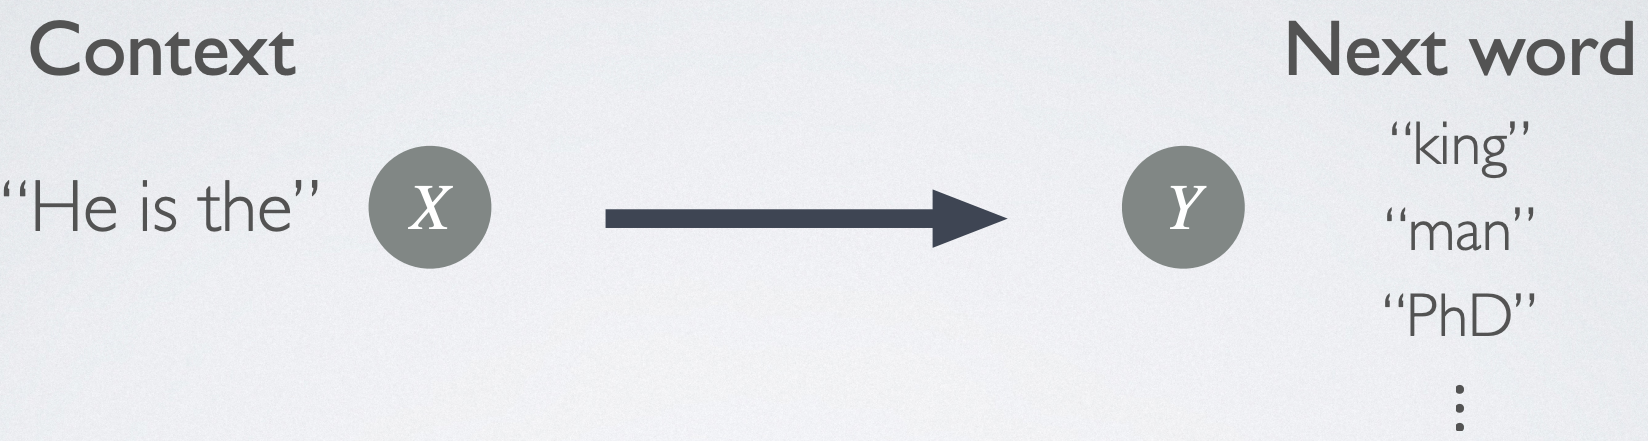
\includegraphics[keepaspectratio]{llm_background.png}}

\paragraph{Embedding}\label{embedding}

\(\lambda(x) \in \mathbb{R}^d\)

\paragraph{Softmax}\label{softmax}

\(\mathbb{P}(y \mid x) \propto \exp(\lambda(x)^\top \gamma(y))\)

\paragraph{Unembedding}\label{unembedding}

\(\gamma(y) \in \mathbb{R}^d\)

Source:
\href{https://kihopark.github.io/files/NeurIPS\%202023\%20Workshop\%20keynote.pdf}{Author's
presentation}

\subsection{Linear Representation
Hypothesis}\label{linear-representation-hypothesis}

The \emph{linear representation hypothesis} suggests that semantic
concepts are linear directions in the model's representation space.

\begin{center}
\pandocbounded{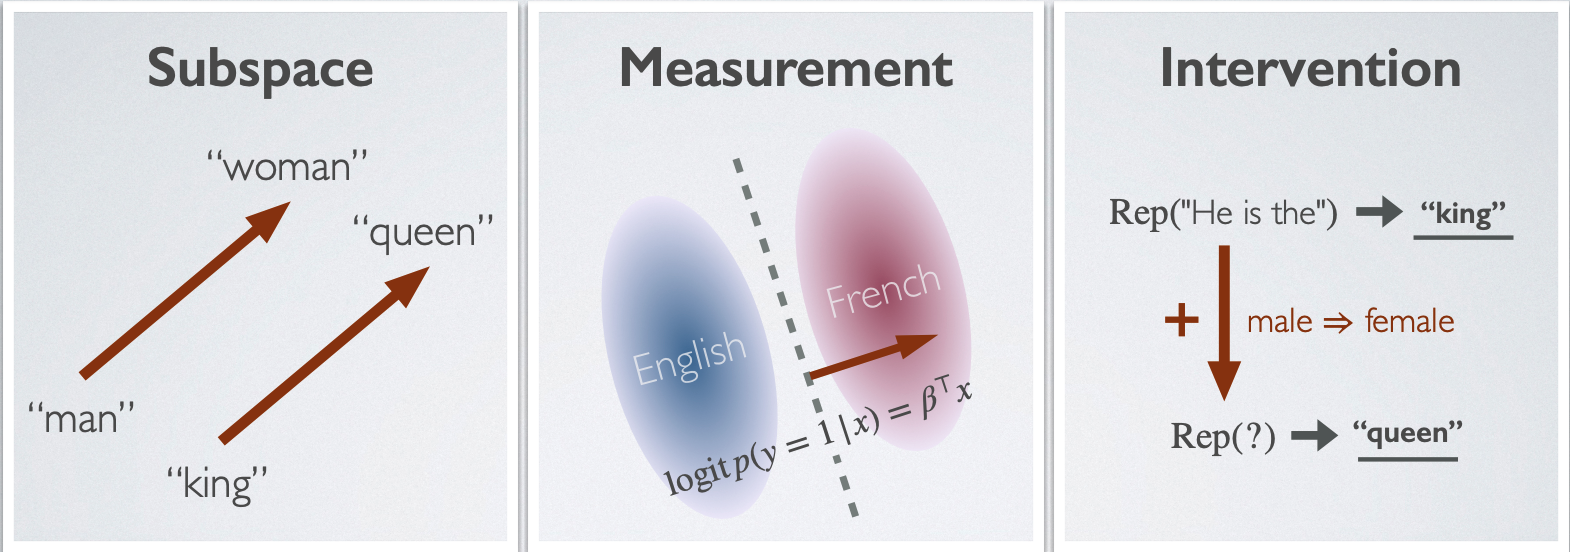
\includegraphics[keepaspectratio]{linear_rep.png}}
\end{center}

Source:
\href{https://kihopark.github.io/files/NeurIPS\%202023\%20Workshop\%20keynote.pdf}{Author's
presentation}

\subsection{Causally Separable
Concepts}\label{causally-separable-concepts}

\pandocbounded{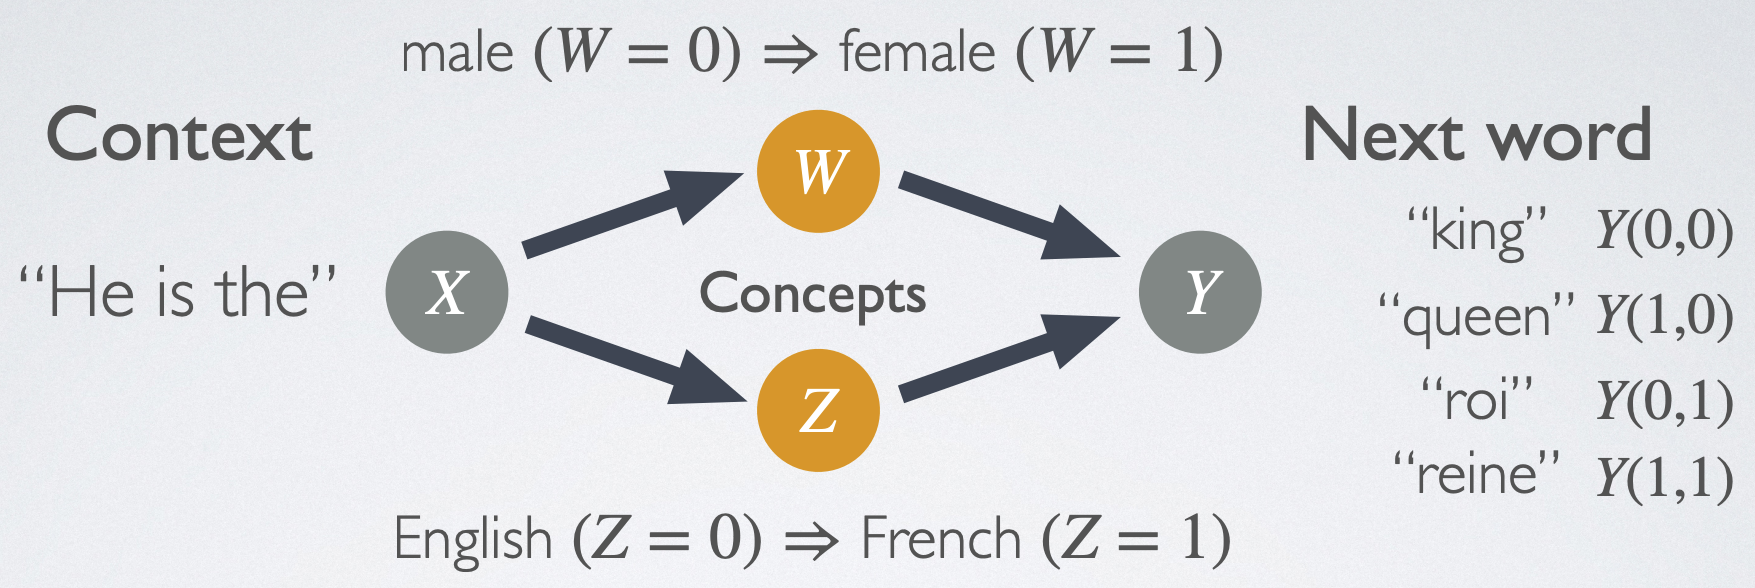
\includegraphics[keepaspectratio]{causally_separable.png}}

Intuition: If two concepts are causally separable, modifying one would
not modify the other one.

Source:
\href{https://kihopark.github.io/files/NeurIPS\%202023\%20Workshop\%20keynote.pdf}{Author's
presentation}

\subsection{Causal Inner Product}\label{causal-inner-product}

\begin{center}
\pandocbounded{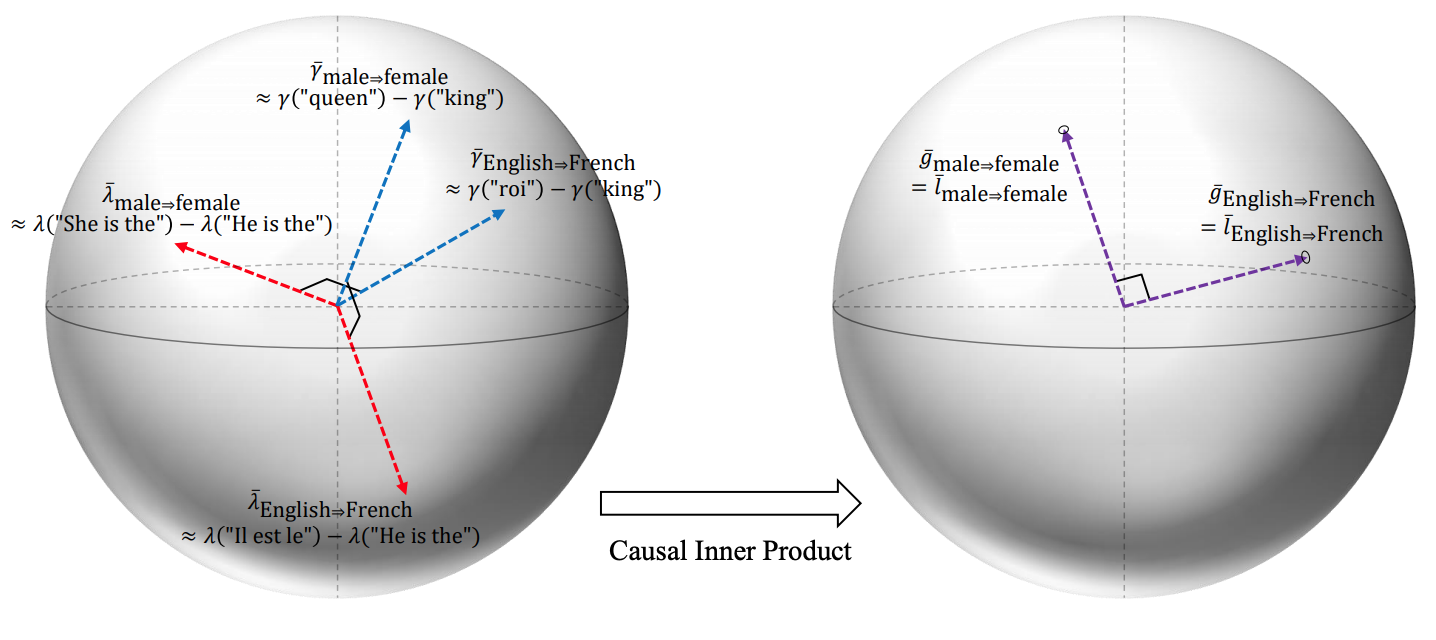
\includegraphics[keepaspectratio]{causal_ip.png}}
\end{center}

\begin{itemize}
\tightlist
\item
  \(\lambda\) is in the embedding space.
\item
  \(\gamma\) is in the unembedding space.
\item
  Intuition: causal inner product induces a linear transformation for
  the representation spaces s.t. causally separable concepts are
  orthogonal.
\item
  The causal inner product unifies \(\bar{g}_W\) (unembedding
  representation of \(W\)) and \(\bar{l}_W\) (embedding representation
  of \(W\)).
\end{itemize}

Source: Park, K., Choe, Y. J., \& Veitch, V. (2023)

\section{General Concepts and Hierarchical
Structure}\label{general-concepts-and-hierarchical-structure}

\subsection{Binary and Categorical
Concepts}\label{binary-and-categorical-concepts}

\pandocbounded{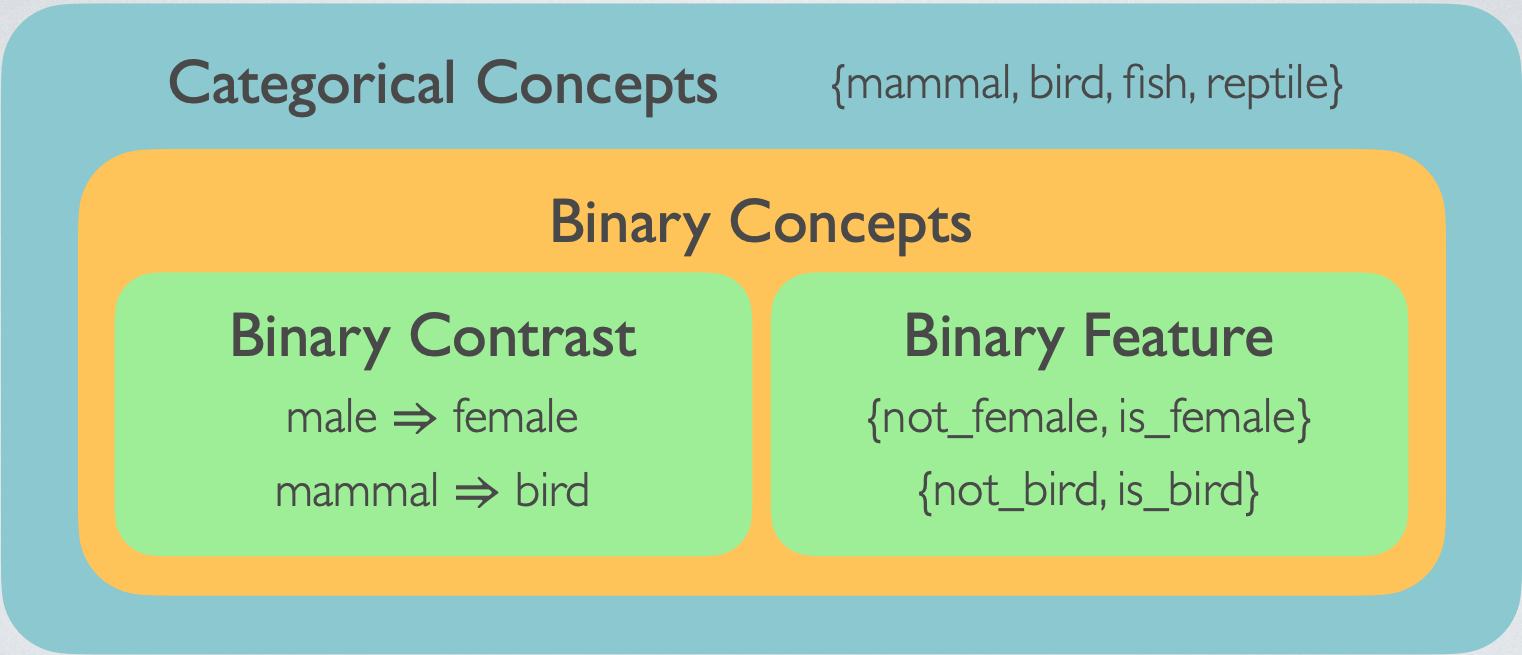
\includegraphics[keepaspectratio]{binary_concepts.png}}

Source:
\href{https://kihopark.github.io/files/ICML\%202024\%20Workshop\%20keynote.pdf}{Author's
presentation}

\subsection{Hierarchical Structure of
Concepts}\label{hierarchical-structure-of-concepts}

\begin{itemize}
\tightlist
\item
  Each attribute \(w\) is associated to a set of tokens
  \(\mathcal{Y}(w)\) that have the attribute.

  \begin{itemize}
  \tightlist
  \item
    For example, \(\mathcal{Y}(\texttt{mammal}) =\) \{``dogs'',
    ``cats'', ``tiger'', \ldots\}.
  \end{itemize}
\end{itemize}

\begin{itemize}
\tightlist
\item
  A value \(z\) is subordinate to a value \(w\) (denoted by
  \(z \prec w\)) if \(\mathcal{Y}(z) \subseteq \mathcal{Y}(w)\).
\end{itemize}

\begin{itemize}
\tightlist
\item
  A categorical concept \(Z \in \{z_0, \ldots, z_{n-1}\}\) is
  subordinate to a categorical concept
  \(W \in \{w_0, \ldots, w_{m-1}\}\) if there exists a value \(w_Z\) of
  \(W\) such that each value \(z_i\) of \(Z\) is subordinate to \(w_Z\).
\end{itemize}

Source: Park, K., Choe, Y. J., Jiang, Y., \& Veitch, V (2024)

\subsection{Hierarchical Structure of Concepts: concrete
examples}\label{hierarchical-structure-of-concepts-concrete-examples}

\begin{itemize}
\tightlist
\item
  The binary contrast ~\(Z = \text{dog} \implies \text{cat}\) is
  subordinate to the binary feature
  \(W = \{\text{is_mammal, not_mammal}\}\), ie, \(Z \prec W\).
\item
  The binary contrast ~\(Z' = \text{parrot} \implies \text{eagle}\) is
  subordinate to the categorical concept
  \(W' = \{\text{mammal, bird, fish}\}\), ie, \(Z' \prec W'\).
\end{itemize}

Source: Park, K., Choe, Y. J., Jiang, Y., \& Veitch, V (2024)

\subsection{\texorpdfstring{Linear Representation \(\bar{l}_W\) of a
Binary
Concept}{Linear Representation \textbackslash bar\{l\}\_W of a Binary Concept}}\label{linear-representation-barl_w-of-a-binary-concept}

Desideratum: If a linear representation exists, moving the
representation in this direction should modify the probability of the
target concept \textbf{in isolation}.

\[P(W = 1\ |\ l + \alpha \bar{l}_W) > P (W = 1\ |\ l)\]

\[P(Z\ |\ l + \alpha \bar{l}_W) = P(Z\ |\ l)\]

For all contexts \(l, \alpha > 0\). \(Z\) is subortinate to or causally
separable with \(W\).

Source:
\href{https://kihopark.github.io/files/ICML\%202024\%20Workshop\%20keynote.pdf}{Author's
presentation}

\section{Representations of Complex
Concepts}\label{representations-of-complex-concepts}

\subsection{High Level Strategy}\label{high-level-strategy}

\begin{enumerate}
\def\labelenumi{\arabic{enumi}.}
\tightlist
\item
  Show how to represent binary features as vectors.
\item
  Show how geometry encodes semantic composition.
\item
  Use this to contruct representations of complex concepts.
\end{enumerate}

Source: Park, K., Choe, Y. J., Jiang, Y., \& Veitch, V (2024)

\subsection{Vector representation of binary
features}\label{vector-representation-of-binary-features}

\begin{itemize}
\tightlist
\item
  Assume that there is a linear representation (normalized direction)
  \(\bar{\ell}_W\) of a binary feature \(W\) for an attribute \(w\).
  Then, there is a constant \(b_w > 0\) such that:
\end{itemize}

\(\left\{
\begin{aligned}
\bar{\ell}_W^\top g(y) &= b_w && \text{if } y \in \mathcal{Y}(w) \\
\bar{\ell}_W^\top g(y) &= 0   && \text{if } y \notin \mathcal{Y}(w)
\end{aligned}
\right.\)

\begin{itemize}
\tightlist
\item
  Intuition: if a perfect linear representation of the \emph{animal}
  feature exists, then every token having the animal attribute has
  roughly the same inner product with the representation vector: ``cat''
  is as much \emph{animal} as ``dog''.
\end{itemize}

Source: Park, K., Choe, Y. J., Jiang, Y., \& Veitch, V (2024)

\subsection{Binary Contrasts Are Vector Differences of Binary
Features}\label{binary-contrasts-are-vector-differences-of-binary-features}

\begin{itemize}
\tightlist
\item
  Let \(w_0 \Rightarrow w_1\) be a binary contrast, and suppose there
  exist vector representations \(\bar{\ell}_{w_0}\) and
  \(\bar{\ell}_{w_1}\). Then, the difference
  \(\bar{\ell}_{w_1} - \bar{\ell}_{w_0}\) is a linear representation
  \(\bar{\ell}_{w_0 \Rightarrow w_1}\).
\end{itemize}

Source: Park, K., Choe, Y. J., Jiang, Y., \& Veitch, V (2024)

\subsection{Categorical Concepts
Representation}\label{categorical-concepts-representation}

\begin{itemize}
\tightlist
\item
  Vector space operations can be used to construct representations of
  \textbf{categorical concepts}, e.g.,\\
  \{mammal, reptile, bird, fish\}.
\item
  The polytope representation of a categorical concept
  \(W = \{w_0,\cdots , w_{k−1} \}\) is the convex hull of the vector
  representations of the elements of the concept.
\end{itemize}

\subsection{Categorical Concepts Representation: Convex
Hull}\label{categorical-concepts-representation-convex-hull}

\begin{Shaded}
\begin{Highlighting}[]
\ImportTok{import}\NormalTok{ numpy }\ImportTok{as}\NormalTok{ np}
\ImportTok{import}\NormalTok{ matplotlib.pyplot }\ImportTok{as}\NormalTok{ plt}
\ImportTok{from}\NormalTok{ scipy.spatial }\ImportTok{import}\NormalTok{ ConvexHull}

\CommentTok{\# Generate random 2D points}
\NormalTok{np.random.seed(}\DecValTok{42}\NormalTok{)}
\NormalTok{points }\OperatorTok{=}\NormalTok{ np.random.rand(}\DecValTok{20}\NormalTok{, }\DecValTok{2}\NormalTok{)}

\CommentTok{\# Compute the convex hull}
\NormalTok{hull }\OperatorTok{=}\NormalTok{ ConvexHull(points)}

\CommentTok{\# Plot}
\NormalTok{plt.figure(figsize}\OperatorTok{=}\NormalTok{(}\DecValTok{6}\NormalTok{, }\DecValTok{6}\NormalTok{))}
\NormalTok{plt.plot(points[:,}\DecValTok{0}\NormalTok{], points[:,}\DecValTok{1}\NormalTok{], }\StringTok{\textquotesingle{}o\textquotesingle{}}\NormalTok{, markersize}\OperatorTok{=}\DecValTok{8}\NormalTok{, markerfacecolor}\OperatorTok{=}\StringTok{\textquotesingle{}lightgray\textquotesingle{}}\NormalTok{, markeredgecolor}\OperatorTok{=}\StringTok{\textquotesingle{}black\textquotesingle{}}\NormalTok{)}

\CommentTok{\# Draw the convex hull lines}
\ControlFlowTok{for}\NormalTok{ simplex }\KeywordTok{in}\NormalTok{ hull.simplices:}
\NormalTok{    plt.plot(points[simplex, }\DecValTok{0}\NormalTok{], points[simplex, }\DecValTok{1}\NormalTok{], }\StringTok{\textquotesingle{}b{-}\textquotesingle{}}\NormalTok{, linewidth}\OperatorTok{=}\DecValTok{2}\NormalTok{)}

\NormalTok{plt.plot(points[hull.vertices, }\DecValTok{0}\NormalTok{], points[hull.vertices, }\DecValTok{1}\NormalTok{], }\StringTok{\textquotesingle{}o\textquotesingle{}}\NormalTok{, markeredgewidth}\OperatorTok{=}\DecValTok{2}\NormalTok{, markeredgecolor}\OperatorTok{=}\StringTok{\textquotesingle{}black\textquotesingle{}}\NormalTok{, markerfacecolor}\OperatorTok{=}\StringTok{\textquotesingle{}white\textquotesingle{}}\NormalTok{)  }\CommentTok{\# hull points}
\NormalTok{plt.axis(}\StringTok{\textquotesingle{}equal\textquotesingle{}}\NormalTok{)}
\NormalTok{plt.axis(}\StringTok{\textquotesingle{}off\textquotesingle{}}\NormalTok{)}
\NormalTok{plt.tight\_layout()}
\NormalTok{plt.show()}
\end{Highlighting}
\end{Shaded}

\begin{figure}[H]

\centering{

\pandocbounded{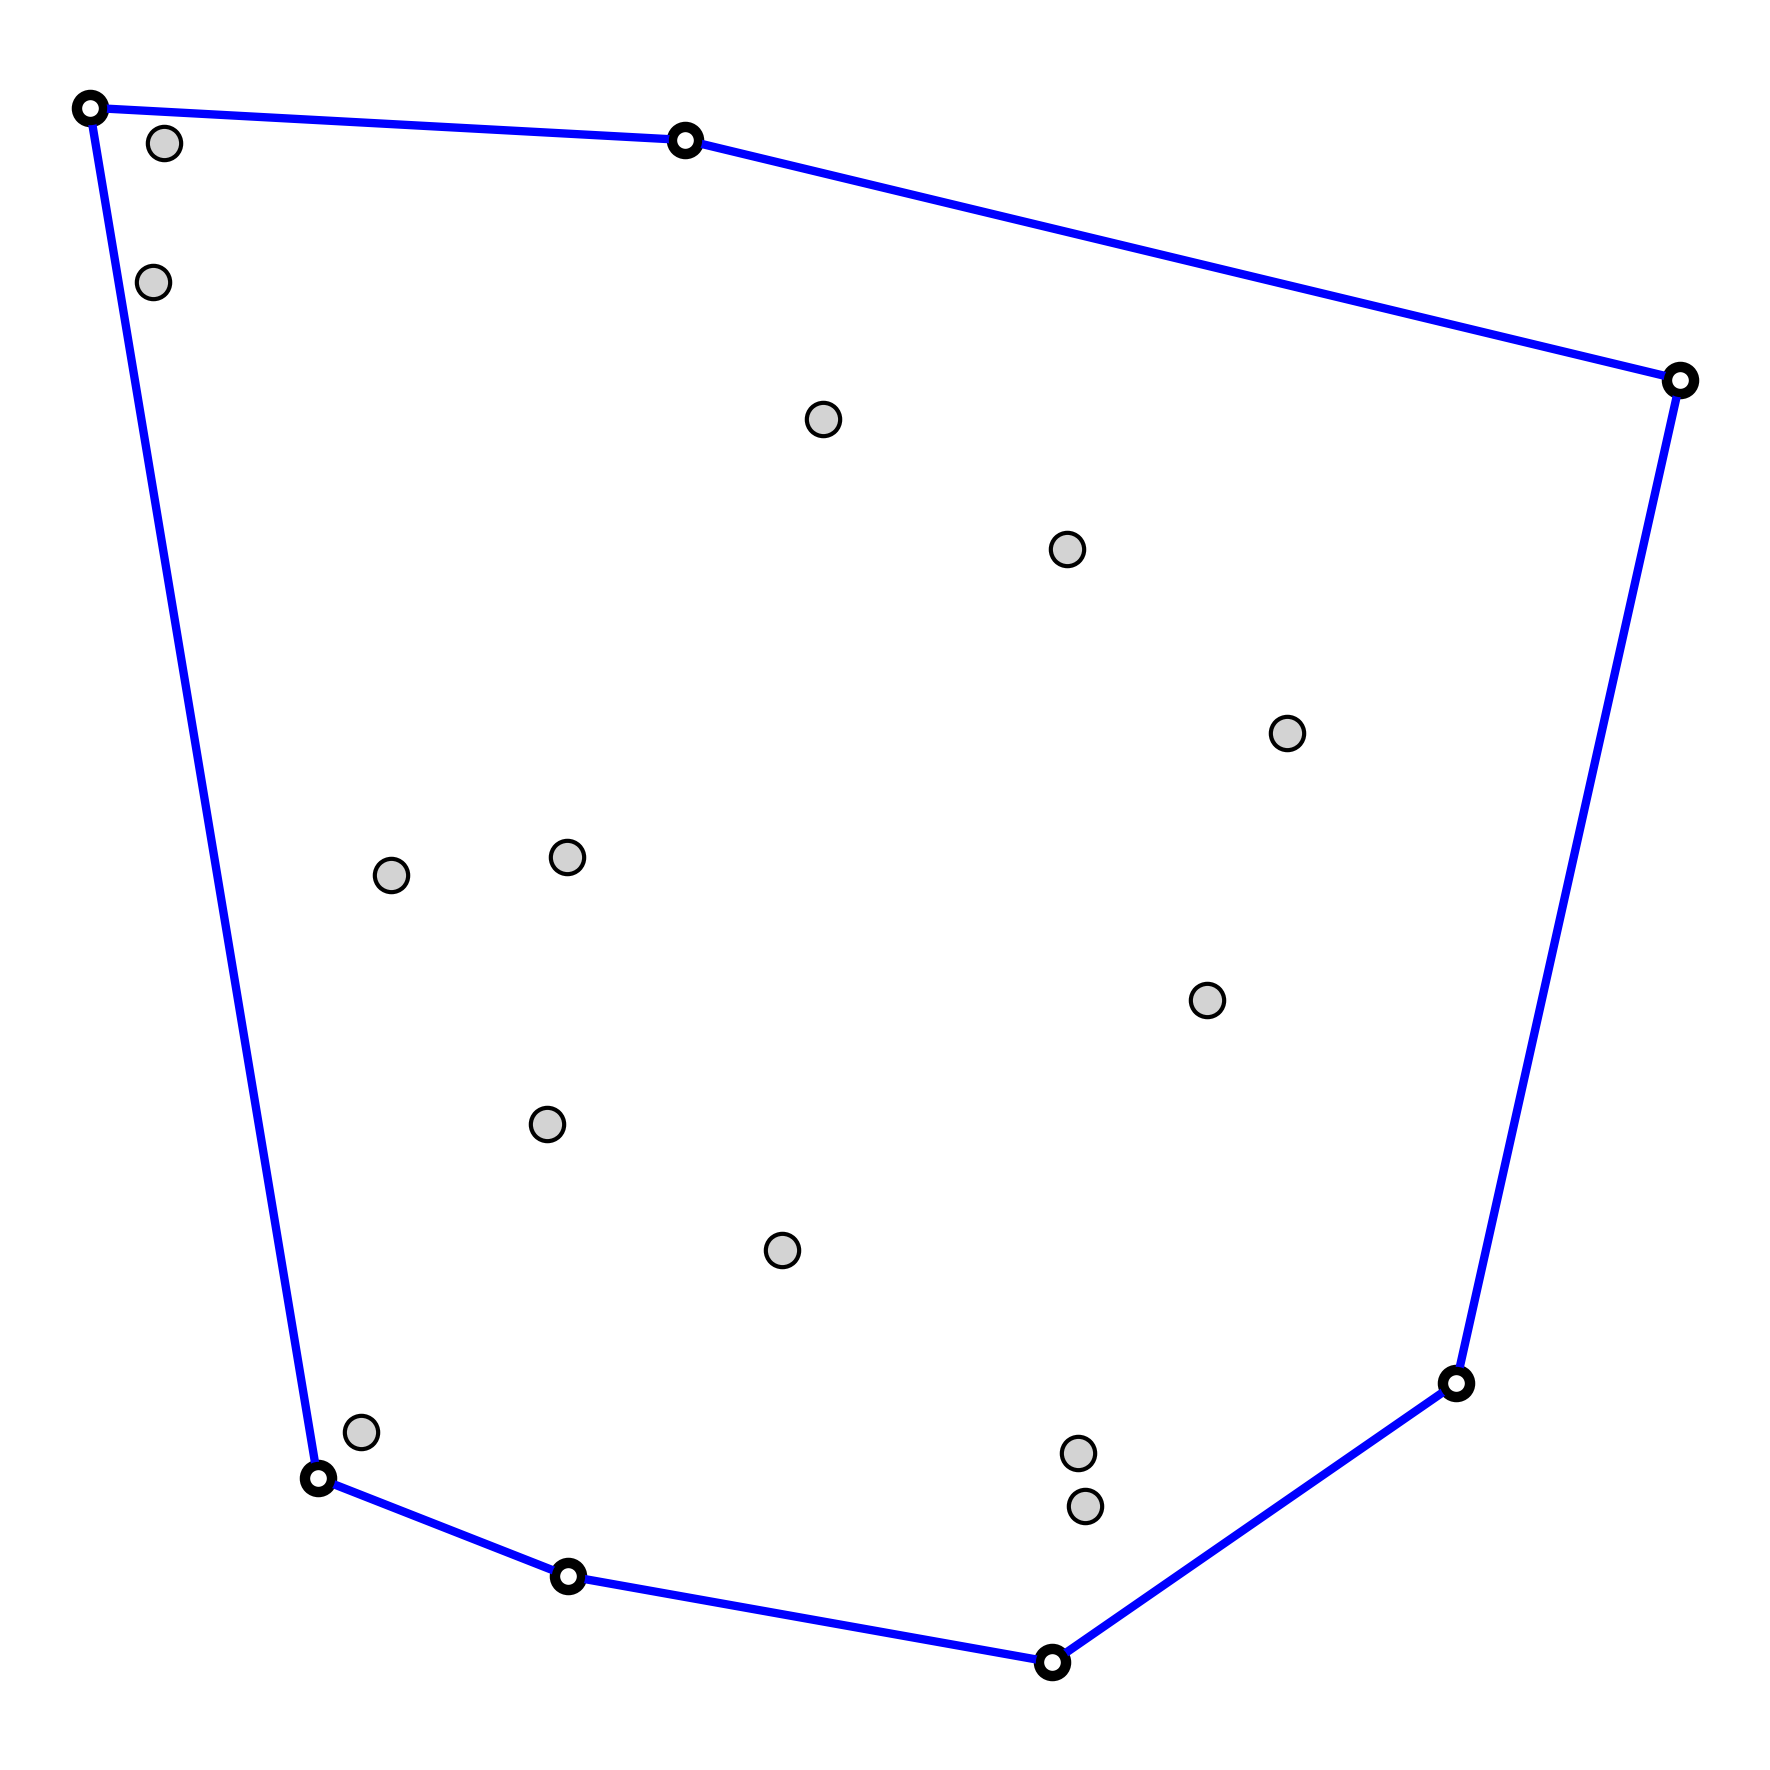
\includegraphics[keepaspectratio]{presentation_files/figure-pdf/fig-polar-output-1.png}}

}

\caption{\label{fig-polar}Convex Hull of Random Points}

\end{figure}%

\subsection{Hierarchical
Orthogonality}\label{hierarchical-orthogonality}

Suppose there exist the vector representations for all the following
binary features. Then, we have that:

\begin{itemize}
\tightlist
\item
  \begin{enumerate}
  \def\labelenumi{(\alph{enumi})}
  \tightlist
  \item
    \(\bar{l}_w \perp \bar{l}_z - \bar{l}_w\) for \(z \prec w\).
  \end{enumerate}
\item
  \begin{enumerate}
  \def\labelenumi{(\alph{enumi})}
  \setcounter{enumi}{3}
  \tightlist
  \item
    \(\bar{l}_{w_1} - \bar{l}_{w_0} \perp \bar{l}_{w_2} - \bar{l}_{w_1}\)
    for \(w_2 \prec w_1 \prec w_0\).
  \end{enumerate}
\end{itemize}

Intuition: Subtracting the parent of the feature gives orthogonality.

\subsection{Hierarchical
Orthogonality}\label{hierarchical-orthogonality-1}

\begin{enumerate}
\def\labelenumi{\alph{enumi}.}
\setcounter{enumi}{1}
\tightlist
\item
  \(\bar{l}_w \perp \bar{l}_{z_0} - \bar{l}_{z_1}\) for
  \(Z \in \{z_0, z_1\}\) subordinate to
  \(W \in \{\textit{not_w}, \textit{is_w}\}\).
\end{enumerate}

\begin{center}
\pandocbounded{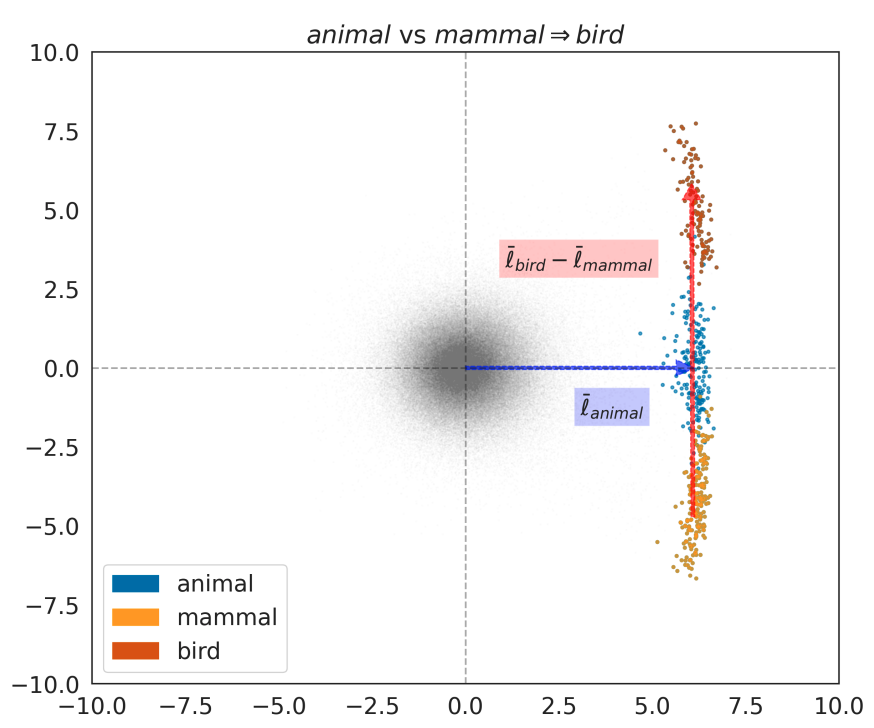
\includegraphics[keepaspectratio]{fig2-b.png}}
\end{center}

Source: Park, K., Choe, Y. J., Jiang, Y., \& Veitch, V (2024)

\subsection{Hierarchical
Orthogonality}\label{hierarchical-orthogonality-2}

\begin{enumerate}
\def\labelenumi{\alph{enumi}.}
\setcounter{enumi}{2}
\tightlist
\item
  \(\bar{l}_{w_1} - \bar{l}_{w_0} \perp \bar{l}_{z_0} - \bar{l}_{z_1}\)
  for \(Z \in \{z_0, z_1\}\) subordinate to \(W \in \{w_0, w_1\}\).
\end{enumerate}

\begin{center}
\pandocbounded{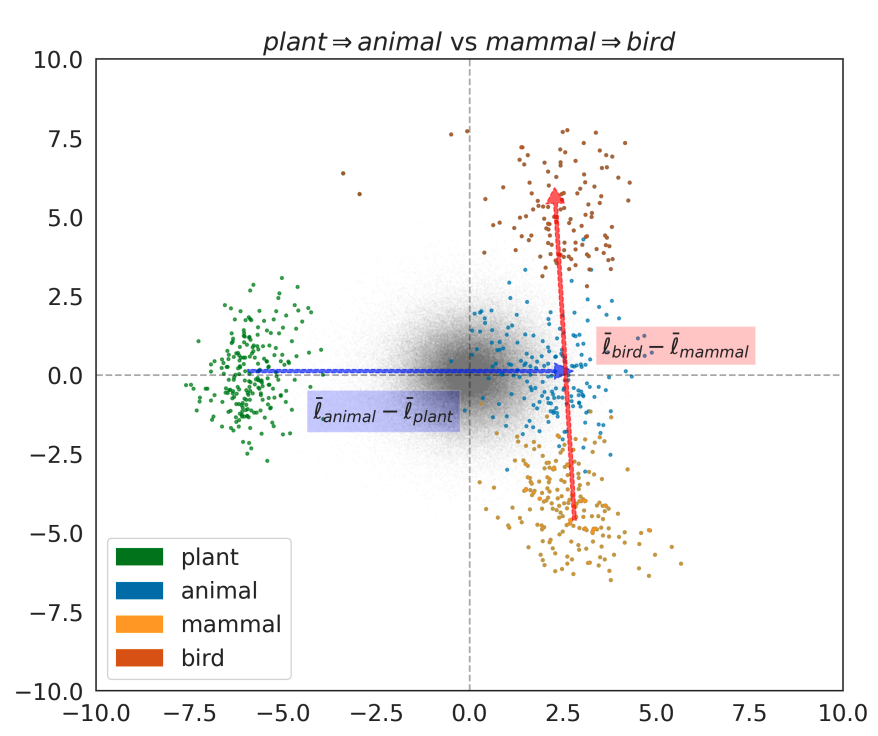
\includegraphics[keepaspectratio]{fig2-c.png}}
\end{center}

Source: Park, K., Choe, Y. J., Jiang, Y., \& Veitch, V (2024)

\section{Some Results}\label{some-results}

\subsection{Setup}\label{setup}

\begin{itemize}
\tightlist
\item
  Gemma-2B model.
\item
  WordNet Dataset:
\end{itemize}

\begin{figure}[H]

{\centering \pandocbounded{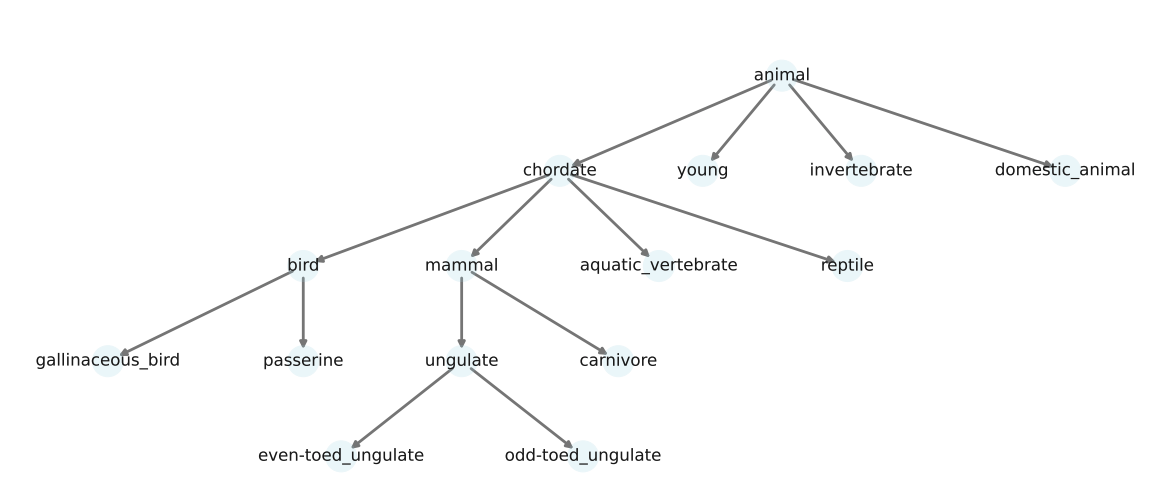
\includegraphics[keepaspectratio]{wordnet_animal_structure.png}}

}

\caption{Subtree in WordNet noun hierarchy for descendants of animal.}

\end{figure}%

Source: Park, K., Choe, Y. J., Jiang, Y., \& Veitch, V (2024)

\subsection{Hierarchical semantics in WordNet are linearly represented
in
Gemma-2B}\label{hierarchical-semantics-in-wordnet-are-linearly-represented-in-gemma-2b}

\begin{itemize}
\tightlist
\item
  The cosine similarity between the vector representations reflects the
  WordNet structure.
\end{itemize}

\begin{figure}[H]

{\centering \pandocbounded{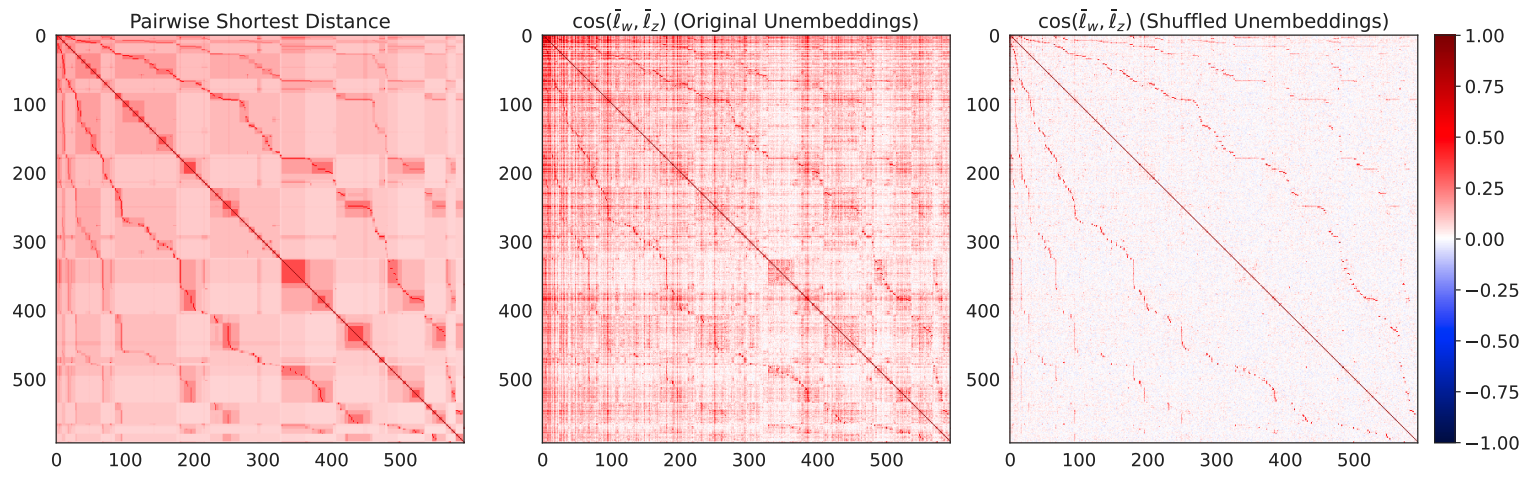
\includegraphics[keepaspectratio]{heatmap.png}}

}

\caption{Heatmaps for the WordNet.}

\end{figure}%

Source: Park, K., Choe, Y. J., Jiang, Y., \& Veitch, V (2024)

\subsection{Hierarchical semantics in WordNet are linearly represented
in
Gemma-2B}\label{hierarchical-semantics-in-wordnet-are-linearly-represented-in-gemma-2b-1}

\begin{figure}[H]

{\centering \pandocbounded{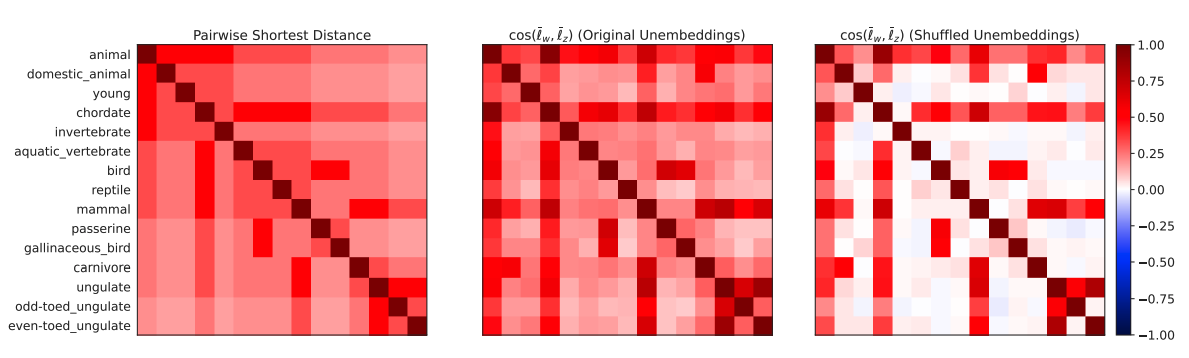
\includegraphics[keepaspectratio]{heatmaps_wordnet_animal.png}}

}

\caption{Heatmaps of the subtree for animal.}

\end{figure}%

Source: Park, K., Choe, Y. J., Jiang, Y., \& Veitch, V (2024)

\subsection{Categorical Concepts are Represented as Polytopes in
Gemma}\label{categorical-concepts-are-represented-as-polytopes-in-gemma}

\begin{center}
\pandocbounded{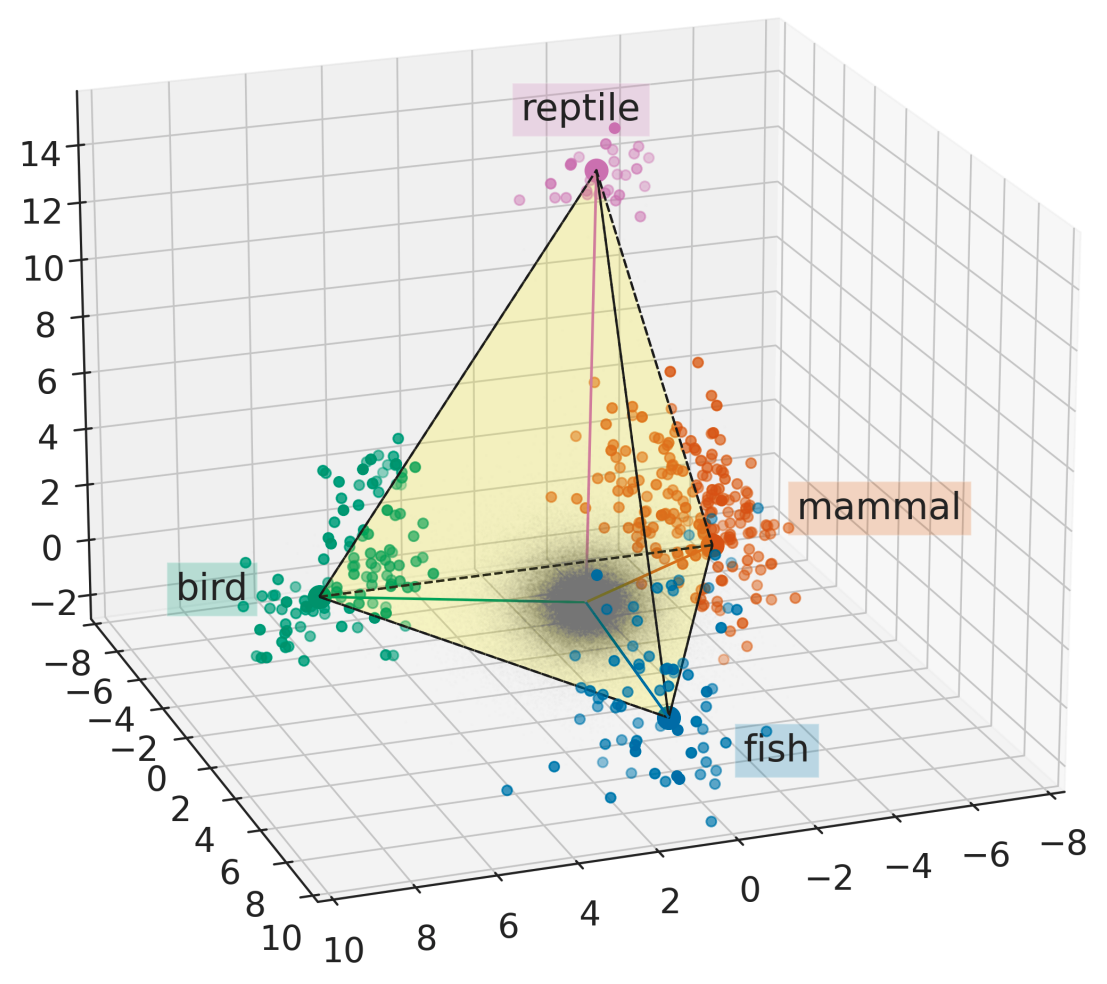
\includegraphics[keepaspectratio]{cat_conceps_poly.png}}
\end{center}

Source: Park, K., Choe, Y. J., Jiang, Y., \& Veitch, V (2024)

\subsection{Overall Structure of the Representation of Hierarchically
Related
Concepts}\label{overall-structure-of-the-representation-of-hierarchically-related-concepts}

\begin{center}
\pandocbounded{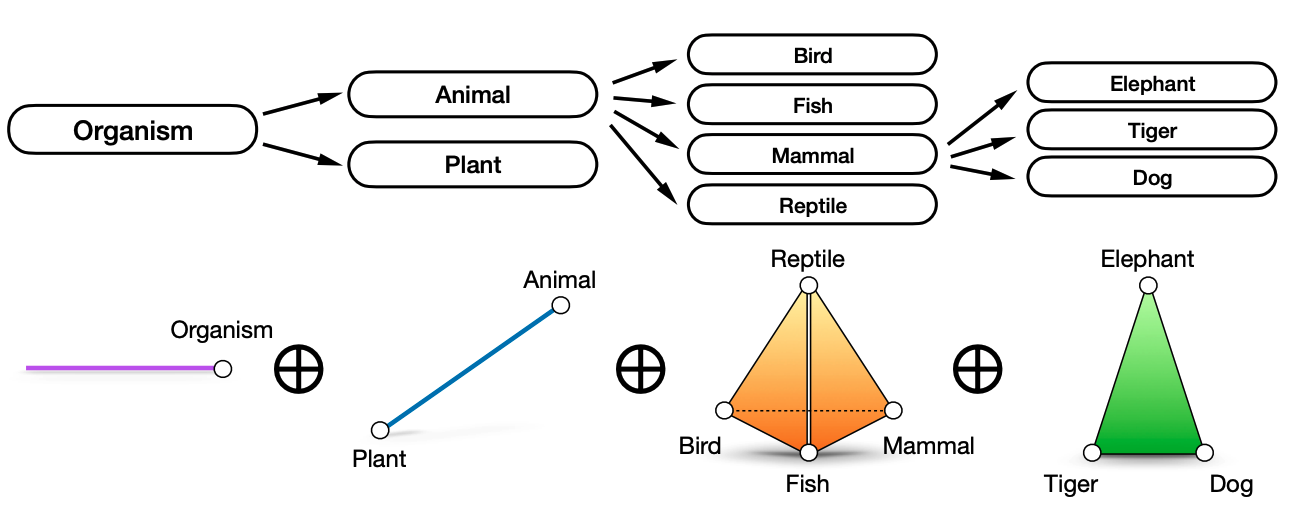
\includegraphics[keepaspectratio]{hierarc_concepts.png}}
\end{center}

Source: Park, K., Choe, Y. J., Jiang, Y., \& Veitch, V (2024)

\section{Q\&A}\label{qa}

\subsection{References}\label{references}

\begin{itemize}
\item
  Park, K., Choe, Y. J., \& Veitch, V. (2024, July). The Linear
  Representation Hypothesis and the Geometry of Large Language Models.
  In International Conference on Machine Learning (pp.~39643-39666).
  PMLR.
\item
  Park, K., Choe, Y. J., Jiang, Y., \& Veitch, V. The Geometry of
  Categorical and Hierarchical Concepts in Large Language Models. In
  ICML 2024 Workshop on Theoretical Foundations of Foundation Models.
\end{itemize}




\end{document}
